\section{\large Аналитические раздел}

В данном разделе рассмотрены технологии thread poll и сокеты poll.

\subsection{Thread pool}

Параллельные вычисления --- это тип вычислений, при котором одновременно выполняется множество операций или процессов.
Пул потоков (Thread pool) \cite{ThreadPools} --- это фиксированный набор потоков, одновременно выполняющих независимые друг от друга задача,
помещенные в массив.
Массив задач представляется в виде очереди.
Ключевым аспектом логики пула потоков является факт того, что все потоки запускаются один раз.

Число операций, которые можно поставить в очередь в пуле потоков, ограничено только доступной памятью.
Однако пул потоков имеет ограничение на число потоков, которые можно активировать в процессе одновременно.
Если все потоки в пуле заняты, дополнительные рабочие элементы помещаются в очередь и ожидают их освобождения.

\begin{figure}[ht!]
	\centering
	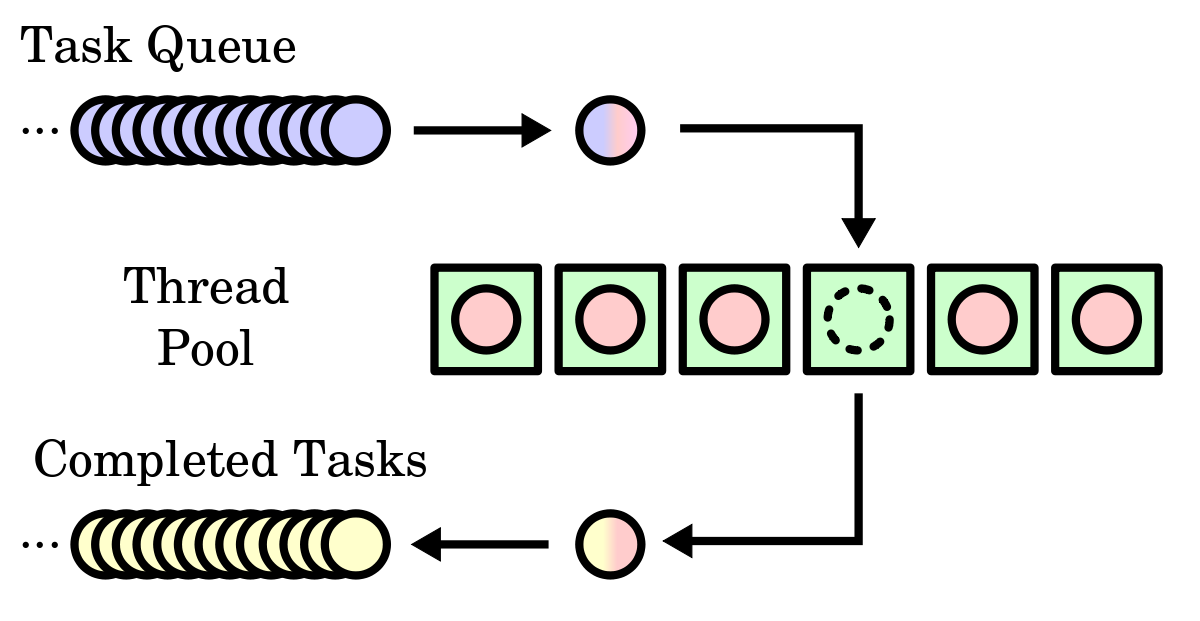
\includegraphics[width=0.7\linewidth]{assets/images/1200px-Thread_pool.svg.png}
	\caption{Thread pool}
	\label{aaa:anal}
\end{figure}
\FloatBarrier

\subsection{Сокет poll}

Сокеты --- название программного интерфейса для обеспечения обмена данными между процессами.
Процессы при таком обмене могут исполняться как на одной ЭВМ, так и на различных, связанных между собой сетью.
Сокет --- это абстрактный объект, представляющий конечную точку соединения.

Каждый сокет имеет свой адрес.
ОС семейства UNIX могут поддерживать много типов адресов, но обязательным являются INET-адрес и UNIX-адрес.

Poll --- этом метод опроса сокетов, созданный после того как ресурсов select оказалось недостаточно.
Преимуществами poll сокетов являются:
\begin{enumerate}
    \item нет никакого лимита количества наблюдаемых дескрипторов;
    \item не модифицируется структура pollfd, что дает возможно ее переиспользования между вызовами poll();
    \item для идентификации отключения клиента, нет необходимости чтение данных из сокета.
\end{enumerate}

Сокеты poll использует блокировку ввода-вывода с мультипликсированием, алгоритм работы представлен на рисунке \ref{fig:anal:use-case}.

\begin{figure}[ht!]
	\centering
	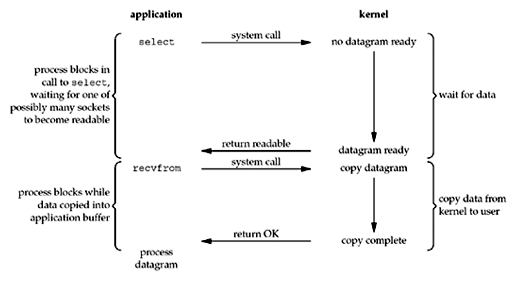
\includegraphics[width=0.7\linewidth]{assets/images/figure_6.3.png}
	\caption{Ввод-вывод с мультипликсированием}
	\label{fig:anal:use-case}
\end{figure}
\FloatBarrier

Основной функцией сокетов является:

\begin{lstlisting}[language=c, label=some-code, caption=Функция poll]
    #include <poll.h>

    int poll (struct pollfd *fdarray, unsigned long nfds, int timeout);
    
    /* Returns: count of ready descriptors, 0 on timeout, –1 on error */
\end{lstlisting}

Первым аргументом этой функции является структура pollfd:

\begin{lstlisting}[language=c, label=some-code, caption=Структура pollfd]
    struct pollfd {
        int     fd;       /* descriptor to check */
        short   events;   /* events of interest on fd */
        short   revents;  /* events that occurred on fd */
      };
\end{lstlisting}

Проверяемые условия задаются членом events, а функция возвращает статус дескритора в соответствующими члене revents.
Такая структура данных (с двумя переменными на дескритор, одна из которых является значением, а другая результатом)
позволяет избежать аргументов <<значение-результат>>.
Каждые из этих двух членов состоит из одного или нескольких битов, которые задают определенное условие.


\subsection*{Вывод}

В данном разделе дано определение пула потоков и сокета poll.
Также был представлен алгоритм их работы.
